\documentclass{beamer}
\usepackage{amsmath}
\usepackage[english]{babel} %set language; note: after changing this, you need to delete all auxiliary files to recompile
\usepackage[utf8]{inputenc} %define file encoding; latin1 is the other often used option
\usepackage{csquotes} % provides context sensitive quotation facilities
\usepackage{graphicx} %allows for inserting figures
\usepackage{booktabs} % for table formatting without vertical lines
\usepackage{textcomp} % allow for example using the Euro sign with \texteuro
\usepackage{stackengine}
\usepackage{wasysym}
\usepackage{tikzsymbols}
\usepackage{textcomp}
% ELIMINAR COMANDOS DE NAVEGACION%%%%%%%%%%%
\setbeamertemplate{navigation symbols}

%\newcommand{\bubblethis}[2]{
 %       \tikz[remember picture,baseline]{\node[anchor=base,inner sep=0,outer sep=0]%
 %       (#1) {\underline{#1}};\node[overlay,cloud callout,callout relative pointer={(0.2cm,-0.7cm)},%
 %       aspect=2.5,fill=yellow!90] at ($(#1.north)+(-0.5cm,1.6cm)$) {#2};}%
 %   }%
%\tikzset{face/.style={shape=circle,minimum size=4ex,shading=radial,outer sep=0pt,
 %       inner color=white!50!yellow,outer color= yellow!70!orange}}

%% Some commands to make the code easier
\newcommand{\emoticon}[1][]{%
  \node[face,#1] (emoticon) {};
  %% The eyes are fixed.
  \draw[fill=white] (-1ex,0ex) ..controls (-0.5ex,0.2ex)and(0.5ex,0.2ex)..
        (1ex,0.0ex) ..controls ( 1.5ex,1.5ex)and( 0.2ex,1.7ex)..
        (0ex,0.4ex) ..controls (-0.2ex,1.7ex)and(-1.5ex,1.5ex)..
        (-1ex,0ex)--cycle;}
\newcommand{\pupils}{
  %% standard pupils
  \fill[shift={(0.5ex,0.5ex)},rotate=80] 
       (0,0) ellipse (0.3ex and 0.15ex);
  \fill[shift={(-0.5ex,0.5ex)},rotate=100] 
       (0,0) ellipse (0.3ex and 0.15ex);}

\newcommand{\emoticonname}[1]{
  \node[below=1ex of emoticon,font=\footnotesize,
        minimum width=4cm]{#1};}
\usepackage{scalerel}
\usetikzlibrary{positioning}
\usepackage{xcolor,amssymb}
\newcommand\dangersignb[1][2ex]{%
  \scaleto{\stackengine{0.3pt}{\scalebox{1.1}[.9]{%
  \color{red}$\blacktriangle$}}{\tiny\bfseries !}{O}{c}{F}{F}{L}}{#1}%
}
\newcommand\dangersignw[1][2ex]{%
  \scaleto{\stackengine{0.3pt}{\scalebox{1.1}[.9]{%
  \color{red}$\blacktriangle$}}{\color{white}\tiny\bfseries !}{O}{c}{F}{F}{L}}{#1}%
}
\usepackage{fontawesome} % Social Icons
\usepackage{epstopdf} % allow embedding eps-figures
\usepackage{tikz} % allows drawing figures
\usepackage{amsmath,amssymb,amsthm} %advanced math facilities
\usepackage{lmodern} %uses font that support italic and bold at the same time

\usepackage{tikz}
\usepackage{tcolorbox}
\usepackage{hyperref}

\usefonttheme[onlymath]{serif} %set math font to serif ones

\definecolor{beamerblue}{rgb}{0.2,0.2,0.7} %define beamerblue color for later use

%%% defines highlight command to set text blue
\newcommand{\highlight}[1]{{\color{blue}{#1}}}


%%%%%%% commands defining backup slides so that frame numbering is correct

\newcommand{\backupbegin}{
   \newcounter{framenumberappendix}
   \setcounter{framenumberappendix}{\value{framenumber}}
}
\newcommand{\backupend}{
   \addtocounter{framenumberappendix}{-\value{framenumber}}
   \addtocounter{framenumber}{\value{framenumberappendix}}
}

%%%% end of defining backup slides

%Specify figure caption, see also http://tex.stackexchange.com/questions/155738/caption-package-not-working-with-beamer
\setbeamertemplate{caption}{\insertcaption} %redefines caption to remove label "Figure".
%\setbeamerfont{caption}{size=\scriptsize,shape=\itshape,series=\bfseries} %sets figure  caption bold and italic and makes it smaller


\usetheme{Boadilla}

%set options of hyperref package
\hypersetup{
    bookmarksnumbered=true, %put section numbers in bookmarks
    naturalnames=true, %use LATEX-computed names for links
    citebordercolor={1 1 1}, %color of border around cites, here: white, i.e. invisible
    linkbordercolor={1 1 1}, %color of border around links, here: white, i.e. invisible
    colorlinks=true, %color links
    anchorcolor=black, %set color of anchors
    linkcolor=beamerblue, %set link color to beamer blue
    citecolor=blue, %set cite color to beamer blue
    pdfpagemode=UseThumbs, %set default mode of PDF display
    breaklinks=true, %break long links
    pdfstartpage=1 %start at first page
    }

\newtcolorbox{boxA}{
    fontupper = \bf,
    boxrule = 1.5pt,
    colframe = black % frame color
}
\newtcolorbox{boxB}{
    boxrule = 1.5pt,
    colframe = blue!70!black,, % frame color
    colback = blue!7!white,
}

% --------------------
% Overall information
% --------------------
\title[Principios de Economía]{Principios de Economía \vspace{4mm} \\
Magistral 1}
\date{}
\author[Riottini]{Franco Riottini}
\vspace{0.4cm}
\institute[]{Universidad de San Andrés} 


\begin{document}

\begin{frame}
\titlepage
\centering

\includegraphics[scale=0.2]{../Figures/logoUDESA.jpg} 
\end{frame}


% \begin{frame}
% \frametitle{Juego de libre asociación}
% \begin{itemize}
%     \item Ingresen a www.menti.com
%     \item Usen el código  1198 4811
%     \item Ingresen 3 palabras que asocien con economía
% \end{itemize} 
%     \begin{center}
%     
\includegraphics[scale=0.2]{../Figures/menti.png}
%     \end{center}
% \end{frame}

\begin{frame}{¿Qué es la economía?}
    \begin{itemize}
        \item Etimología de la palabra economía: del griego \textit{oikos} (casa, patrimonio) y \textit{nemein} (administrar, gestionar) \vspace{2mm}
        \item Es una ciencia: tiene un objeto propio (la asignación de recursos escasos), un método (hipotético - deductivo) y un conjunto de modelos capaces de explicar los fenómenos que se observan en la realidad
        \item Es una ciencia empírica: se puede contrastar con la realidad 
        \item Es una ciencia social: estudia diversos aspectos de las sociedades
        \vspace{2mm}
        \begin{center}
            \begin{boxA}
            La economía es una ciencia empírica y social que se ocupa de la manera en que se administran los recursos escasos
            \end{boxA}
        \end{center}
        \item Definitivamente \textbf{no} es una ciencia exacta
    \end{itemize}
\end{frame}

\begin{frame}{¿Qué hace un economista?}
    \begin{itemize}
        \item Busca asignar eficientemente recursos escasos \vspace{3mm} \\
        \item ¿Que quiere decir ``eficientemente''? Depende del objetivo que tengamos en mente! Pero siempre tendrá que ver con utilizar los recursos de la mejor manera posible (desaprovechando lo menor cantidad posible) \vspace{3mm} \\
        \item ¿Qué mecanismos tiene para realizar dicha asignación? 
        \begin{itemize}
            \item Sorteo?
            \item El que primero levanta la mano?
            \item El que más necesita?
            \item Designar alguien que decida?
            \begin{boxA}
                \begin{center}
                    \textbf{O EL MERCADO !}
                \end{center}
            \end{boxA}
        \end{itemize}
    \end{itemize}
\end{frame}

\begin{frame}
\frametitle{¿Cómo los puedo asignar?}
El color de la persona indica la preferencia por el color de la taza. Supongamos que el mecanismo de asignación es un sorteo.
\begin{center}
    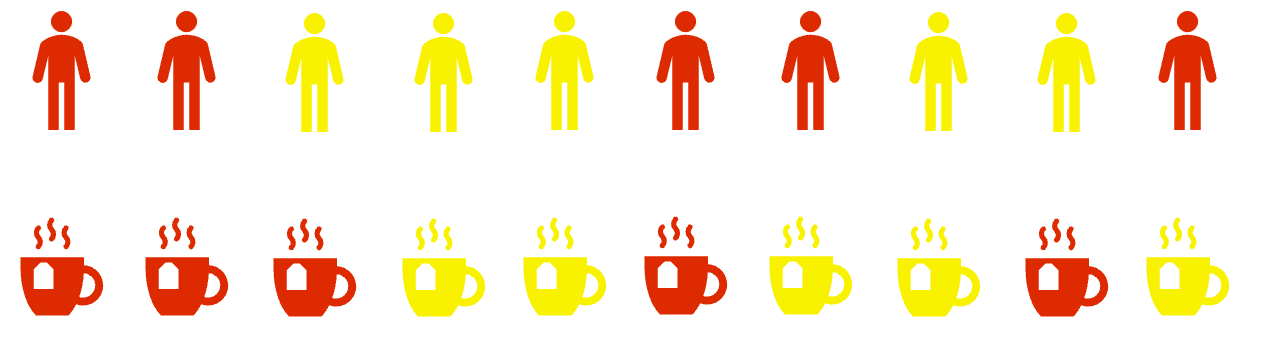
\includegraphics[scale=0.8]{../Figures/Tazon.png}
\end{center}
\begin{itemize}
    \item ¿Es eficiente esta asignación?
    \item ¿Qué pasaría si el mecanismo de asignación fuera un planificador central? ¿A gran escala se puede?
    \item ¿Y un mercado? La gente podría cambiar el que quisiera por uno de su preferencia
\end{itemize}
\end{frame}

\begin{frame}
\frametitle{¿Y ahora?}
    \begin{center}
        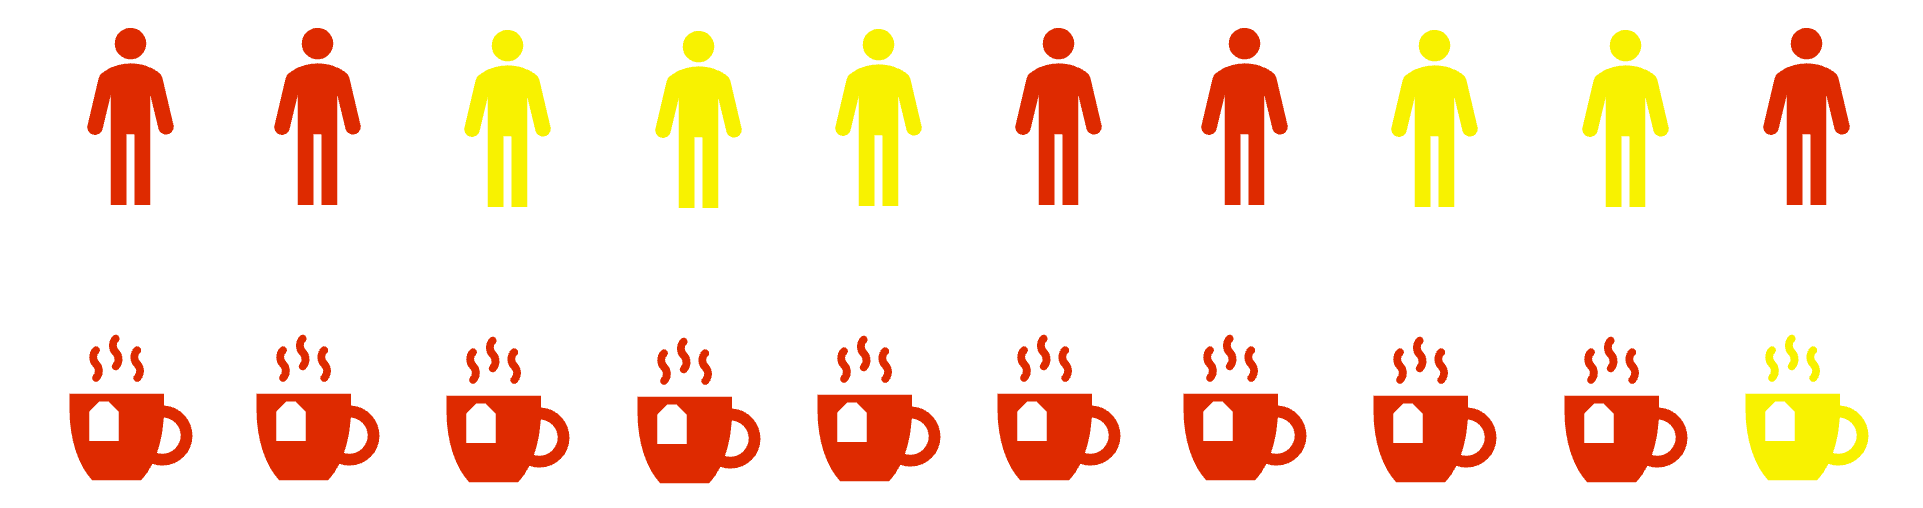
\includegraphics[scale=0.55]{../Figures/Tazon3.png}
    \end{center}
    \begin{itemize}
        \small
        \item La idea de eficiencia es muy relevante ya que implica un win-win
        \begin{center}
            \begin{boxA} 
                \textbf{Los economistas consideran que una asignación es ineficiente cuando podemos mejorar el bienestar de alguien (o de varios) sin perjudicar a otros}
            \end{boxA}
        \end{center}
        \item Ojo: Eficiente no quiere decir justa...
        \item Eficiencia y equidad (distribución) son asuntos distintos para el economista
    \end{itemize}
\end{frame}

\begin{frame}
\frametitle{¿Qué aspectos estudia la economía?}
\begin{itemize}
    \item Cómo tomamos decisiones  \vspace{2mm}
    \item Cómo interactuamos unos con otros (compradores y vendedores, empleados y empleadores, ciudadanos y servidores públicos, padres, hijos y familia) \vspace{2mm}
    \item Cómo interactuamos con nuestro entorno \vspace{2mm}
    \item Cómo estas cosas cambian en el tiempo  
\end{itemize}
\end{frame}

\begin{frame}
\frametitle{Entendiendo el mundo}
Estudiar las causas y consecuencias de los problemas sociales es un reto 
\begin{itemize}
    \item Responder algunas preguntas no es fácil...
    \begin{itemize}
        \item ¿Por qué algunos países son ricos y otros son pobres?
        \item ¿Por qué hay inflación en Argentina?
        \item ¿Las mujeres que se casan más tarde tienen niños más educados?
        \item ¿Causan los cinturones de seguridad más accidentes?
        \end{itemize}
    \item ¡A veces es complicado comprender la pregunta!
\end{itemize}
\end{frame}

\begin{frame}{¿Cómo hacer frente a estas preguntas?}
        \begin{itemize}
                \item Vamos a pensar utilizando modelos económicos... \vspace{2mm}
                \item y vamos confrontar esos modelos con la realidad
        \end{itemize} \vspace{2mm}
    \begin{center}
        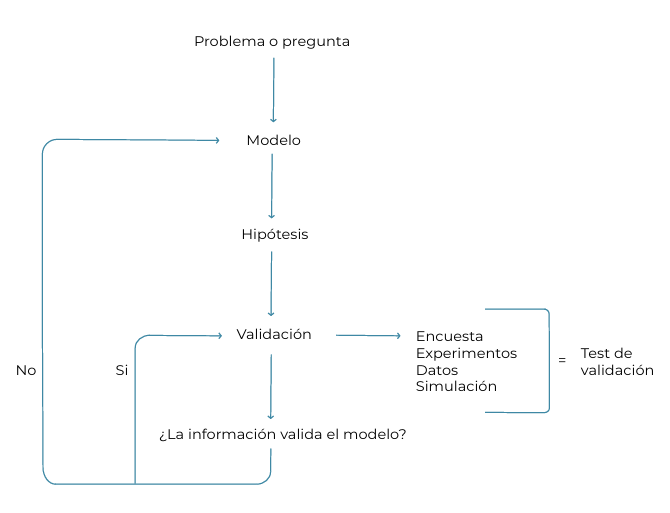
\includegraphics[scale=0.5]{../Figures/C.1.4.png}
    \end{center}
\end{frame}

\begin{frame}{¿Que es un modelo?}
\begin{itemize}
    \item ¡El mundo es muy complejo! Para entenderlo debemos simplificar la realidad \vspace{2mm} \\ $\Rightarrow$
    Supuestos y modelos \vspace{2mm}
    \item Es una simplificación de la realidad \vspace{2mm}
    \item Construimos una descripción simplificada en base a \textbf{la pregunta de interés} 
    \item  \href{https://www.youtube.com/watch?v=zwDA3GmcwJU}{``Del rigor de la ciencia''} 
    Jorge Luis Borges
    \item La conclusión de los modelos requiere derivar conclusiones lógicas de supuestos (utilizando algebra, gráficos, cálculo, etc.)
    \item El formalismo en los modelos no es otra cosa que "asegurar el razonamiento lógico" que nos lleva de los supuestos a las conclusiones.
\end{itemize}
\end{frame}

\begin{frame}
\frametitle{¿Cómo construimos modelos?}
    \begin{itemize}
        \item Determinamos las hipotesis y resultados del modelo 
        \item Validación de una teoría: comparación de sus predicciones con la realidad.
        \item Nunca podemos afirmar que una hipótesis es cierta porque esté de acuerdo con los hechos.
        \item Si podemos negar la verdad de una hipótesis en base a ellos.
        \item “No existe lógica de la verificación, sí de la refutación” (Blaug).
        \begin{center}
            \begin{boxA}
                \textbf{Una teoría estará bien corroborada, no cuando esté de acuerdo con un gran número de hechos, sino cuando seamos incapaces de encontrar hechos que la refuten. La teoría resiste y se consolida.}
            \end{boxA}
        \end{center}
    \end{itemize}
\end{frame}

\begin{frame}
\frametitle{Modelos y supuestos}
\begin{itemize}
    \item En un sentido estricto, todos los supuestos son irrealistas. No se puede hacer una descripción exacta de la realidad
    \item No hay que examinar el grado de realismo de los supuestos, sino su utilidad para entender la realidad
    \item Muchas veces esta utilidad radica en la capacidad de, luego derivadas las conclusiones, modificar los supuestos para ver como se modifican esas conclusiones
    \begin{center}
        \begin{boxA}
            \textbf{“Criticar los modelos económicos por sus supuestos irrealistas es como criticar los experimentos de la bola rodante de Galileo por utilizar un plano perfeccionado para tener la menor fricción posible” (Nancy Cartwright)}
        \end{boxA}
    \end{center}
    
\end{itemize}
\end{frame}

\begin{frame}
\frametitle{¿Qué es un buen modelo?}
\begin{itemize}
    \item El que nos ayuda a entender algo importante
    \item Predice con precisión: sus predicciones son consistentes con la evidencia \vspace{1mm}
    \item Mejora la comunicación. Nos ayuda a entender en qué estamos de acuerdo (y qué en desacuerdo) \vspace{1mm}
    \item Es útil. Podemos usarlo para encontrar formas de mejorar el funcionamiento de la economía
\end{itemize} 
\end{frame}

\begin{frame}
\frametitle{¿Por qué vamos a usar gráficos?}
\begin{itemize}
    \item Los gráficos sirven para mostrar ideas \vspace{2mm}
    \item Los gráficos son útiles para ver si hay relación entre dos variables 
     \begin{itemize}
        \item ¡Pero tenemos que tener cuidado! Esas relaciones dan indicios de correlación... pero no de causalidad! \vspace{2mm}
    \end{itemize}
    \item Los gráficos (y sus expresiones matemáticas) pueden ser utilizados para describir una teoría
\end{itemize} 
\end{frame}

\begin{frame}
\frametitle{La correlación...}
\begin{center}
    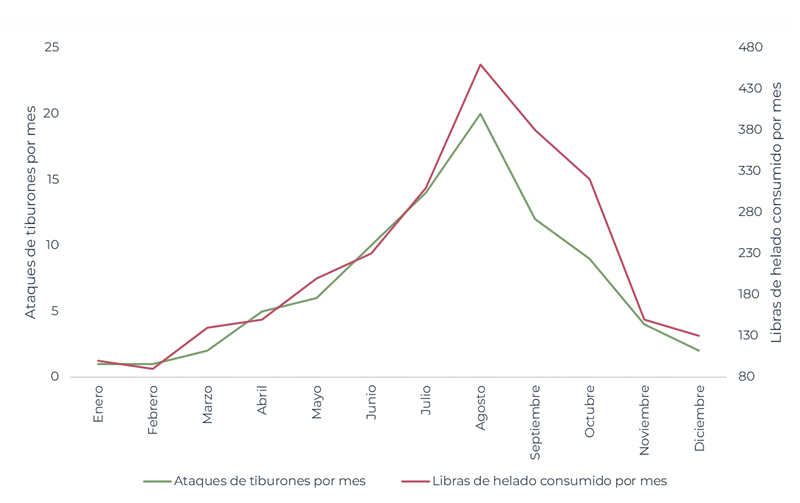
\includegraphics[scale=0.55]{../Figures/C2.13.png}
\end{center}
\end{frame}

\begin{frame}
    \frametitle{Algunas explicaciones}
    \begin{itemize}
        \item OJO al interpretar relaciones entre variables porque \textcolor{blue}{correlación no implica causalidad} 
        \begin{boxB}
        \textbf{Correlación}: relación recíproca entre dos o más acciones, variables o fenómenos. \\
        \textbf{Causalidad}: relación causa-efecto. Hay causalidad si mover una variable x genera un cambio en la variable y.
        \end{boxB}
        \item Endogeneidad: ``todo tiene que ver con todo'' \vspace{1mm}
        \begin{itemize} 
         \item ¿En qué sentido va la correlación?
            \item Potenciales fuentes de confusión:
            \begin{itemize}
                \item {Omisión de variables}  
                \item {Simultaneidad} 
                \item {Error de medición en la variable explicativa}
            \end{itemize}
        \end{itemize}
    \end{itemize}
\end{frame}

\begin{frame} 
    \frametitle{¿Qué podemos hacer?}
    \begin{itemize}
        \item  En algunos casos se pueden diseñar experimentos o utilizar experimentos naturales (exógenos por definición) para detectar eventos que producen un cambio claro en una variable (algunos ejemplos \hyperlink{appendix}{acá})
        \item Usamos técnicas estadísticas que nos permitan "descubrir" la causalidad a partir los datos que tenemos. Para ello usamos algo que los economistas llaman "econometría". 
    \end{itemize}
\end{frame}

\begin{frame}
    \begin{center}
        \LARGE  \textbf{IMPORTANTE}  \\ \vspace{1cm}
        \Large 
        \begin{boxB}
        \centering Leer capítulos 2, 3 y 4 de esta clase
        \end{boxB}
        \vspace{0.5cm}
        \begin{boxB}
        Leer capítulos 5 y 6 para el viernes - HAY QUIZ!
        \end{boxB}
    \end{center}
\end{frame}

\begin{frame} \label{appendix}
    \frametitle{Experimentos}
    \begin{center}
    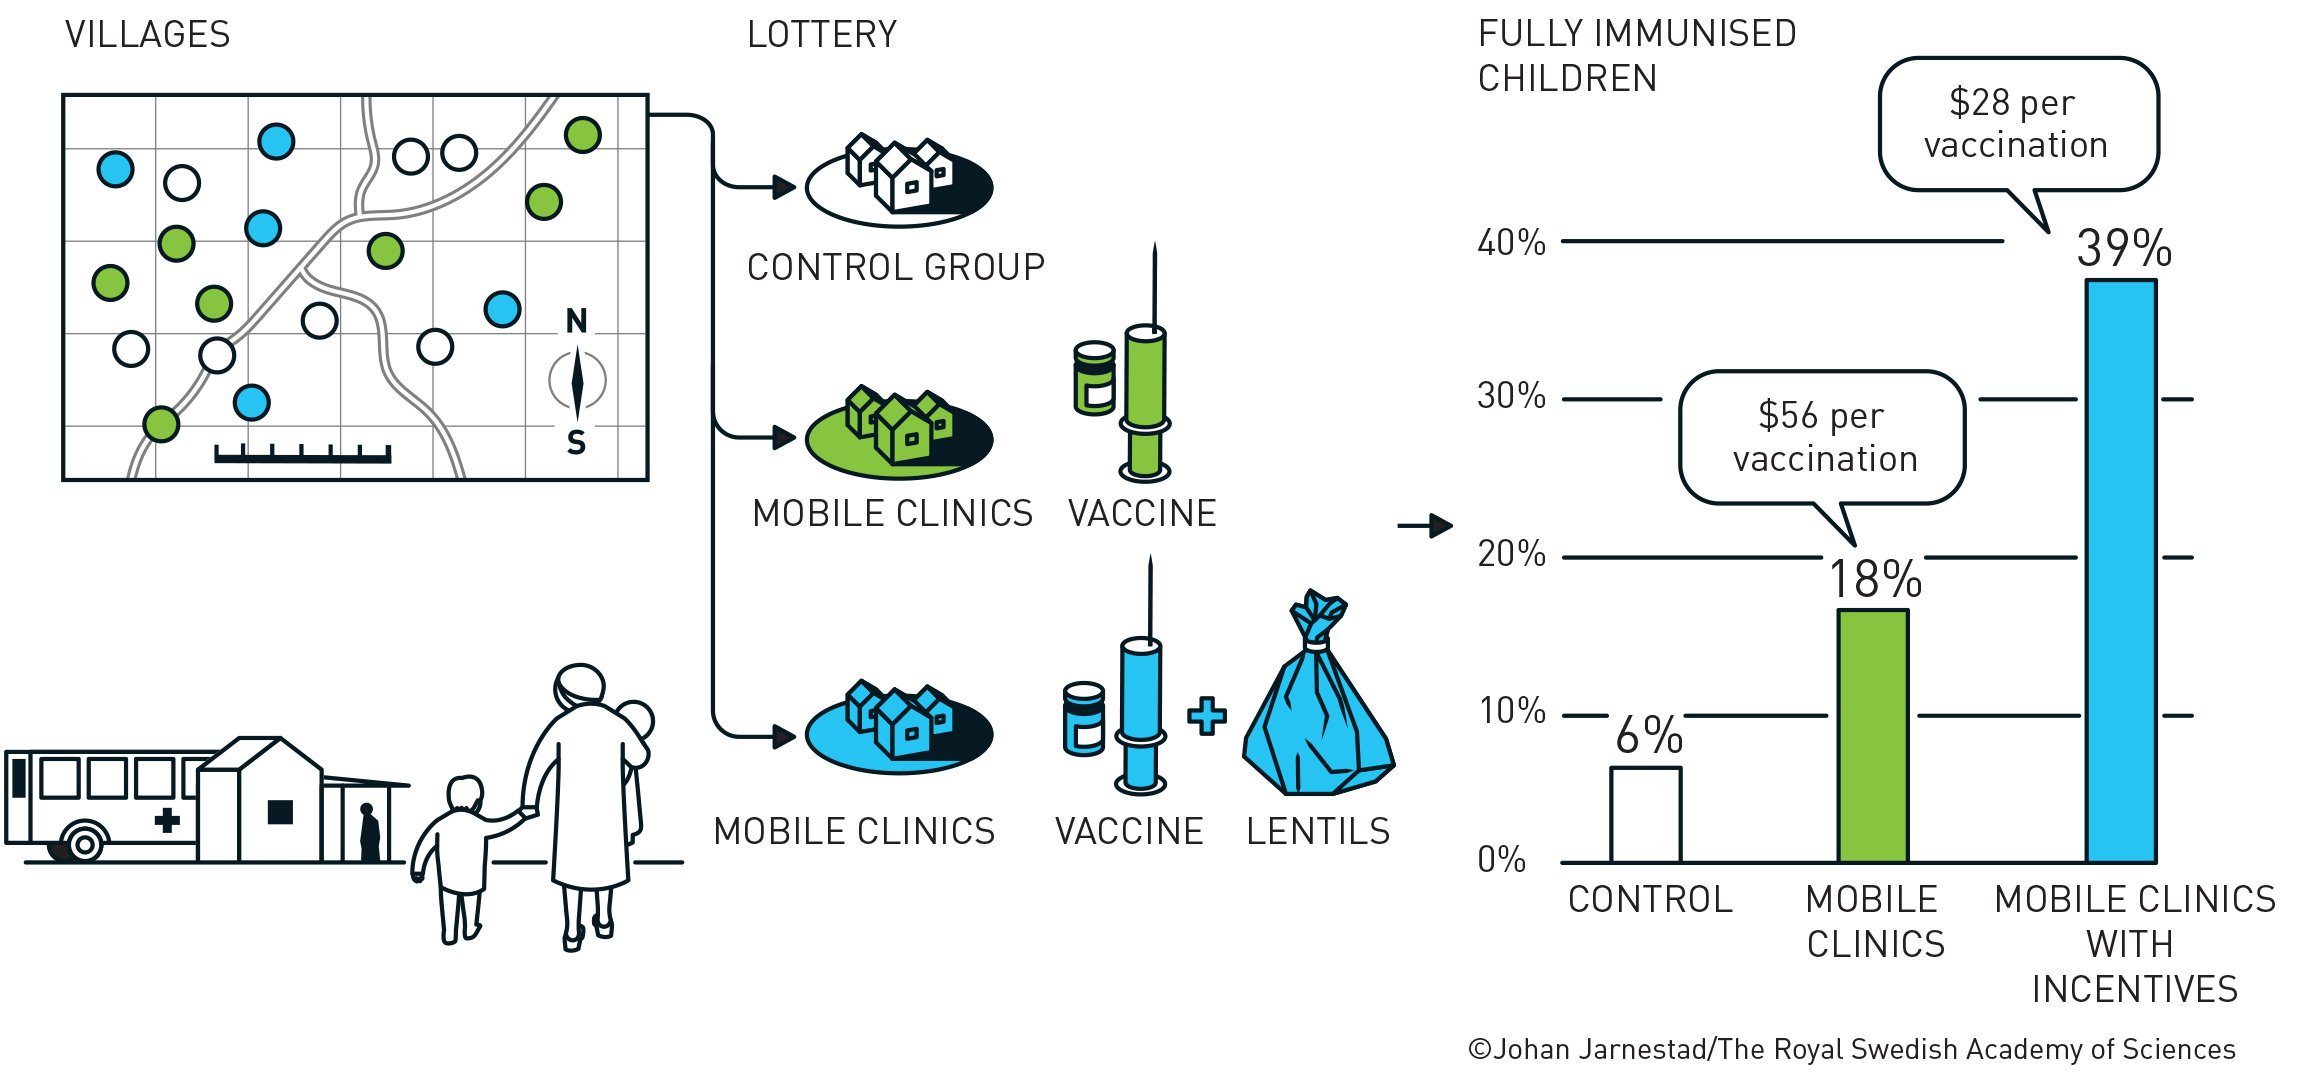
\includegraphics[scale=0.1]{Slides Principios de Economia/Figures/rct_vacunas.png}
    \end{center}
    “Improving immunisation coverage in rural India: clustered randomised controlled evaluation of immunization campaigns with and without incentives” - Banerjee, Duflo, Glennerster \& Kothari (2010) \\  \vspace{2mm}
\end{frame}
    
\begin{frame} 
    \frametitle{Experimentos naturales}
    \begin{center}
        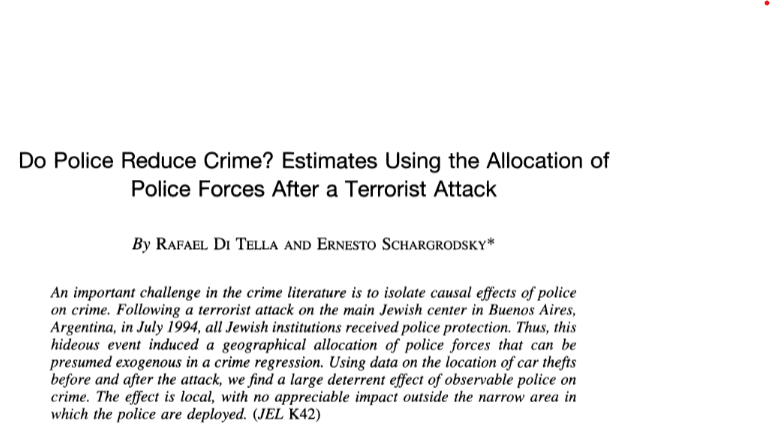
\includegraphics[scale=0.5]{../Figures/Do_Police_Induce_Crime.png}
    \end{center}
\end{frame}

\end{document}
